\documentclass{article}
\usepackage{tikz}
\usetikzlibrary{decorations.pathreplacing}

\begin{document}

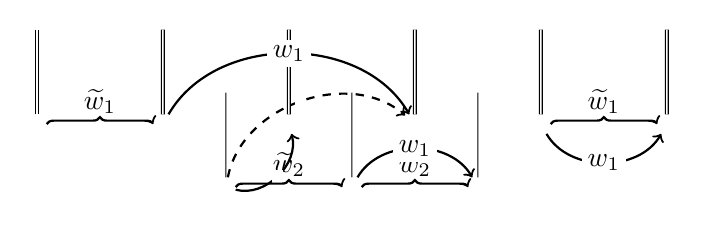
\begin{tikzpicture}[scale=0.8]
    % Define nodes for the diagram
    \node (A) at (0,0) {};
    \node (B) at (2,0) {};
    \node (C) at (4,0) {};
    \node (D) at (6,0) {};
    \node (E) at (8,0) {};
    \node (F) at (10,0) {};

    \node (G) at (3,-1) {};
    \node (H) at (5,-1) {};
    \node (I) at (7,-1) {};

    \draw[double] (A) -- ++(0,1.5);
    \draw[double] (B) -- ++(0,1.5);
    \draw[double] (C) -- ++(0,1.5);
    \draw[double] (D) -- ++(0,1.5);
    \draw[double] (E) -- ++(0,1.5);
    \draw[double] (F) -- ++(0,1.5);

    \draw (G) -- ++(0,1.5);
    \draw (H) -- ++(0,1.5);
    \draw (I) -- ++(0,1.5);

    % Draw the connections
    \draw[->, decoration={brace}, decorate, thick] (A) -- node[above] {$\widetilde{w}_1$} (B);
    \draw[->, decoration={brace}, decorate, thick] (E) -- node[above] {$\widetilde{w}_1$} (F);
    \draw[->, decoration={brace}, decorate, thick] (G) -- node[above] {$\widetilde{w}_2$} (H);
    \draw[->, decoration={brace}, decorate, thick] (H) -- node[above] {$\widetilde{w}_2$} (I);

    % Draw the skip connections
    \draw[->, bend left=60, thick] (B) to node[fill=white, inner sep=2pt] {$w_1$} (D);
    \draw[->, bend right=60, thick] (E) to node[fill=white, inner sep=2pt] {$w_1$} (F);
    \draw[->, bend left=60, thick] (H) to node[fill=white, inner sep=2pt] {$w_1$} (I);
    \draw[->, dashed, bend left=60, thick] (G) to node[fill=white, inner sep=2pt] {} (D);
    \draw[->, bend right=60, thick] (G) to node[fill=white, inner sep=2pt] {} (C);
\end{tikzpicture}

\end{document}